%%%%%%%%%%%%%%%%%%%%%%%%%%%%%%%%%%%%%%%%%%%%%%%%%%%%%%%%%%%%%%%%%%%%%%
%     File: ExtendedAbstract_intro.tex                               %
%     Tex Master: ExtendedAbstract.tex                               %
%%%%%%%%%%%%%%%%%%%%%%%%%%%%%%%%%%%%%%%%%%%%%%%%%%%%%%%%%%%%%%%%%%%%%%

\section{Introduction}
\label{sec:intro}

Referring Instance Segmentation is a fundamental task in computer vision that requires models to identify and segment specific object instances using natural language descriptions. When applied to aerial photographs, also referred to as Referring Remote Sensing Instance Segmentation (RRSIS), this task represents a major challenge due to the intricate characteristics of aerial imagery, including varying scales and resolutions of top-down perspectives, geographic complexities, extreme object density variations, and unique spatial relationships not present in ground-level photography.

\begin{figure}[H]
\centering
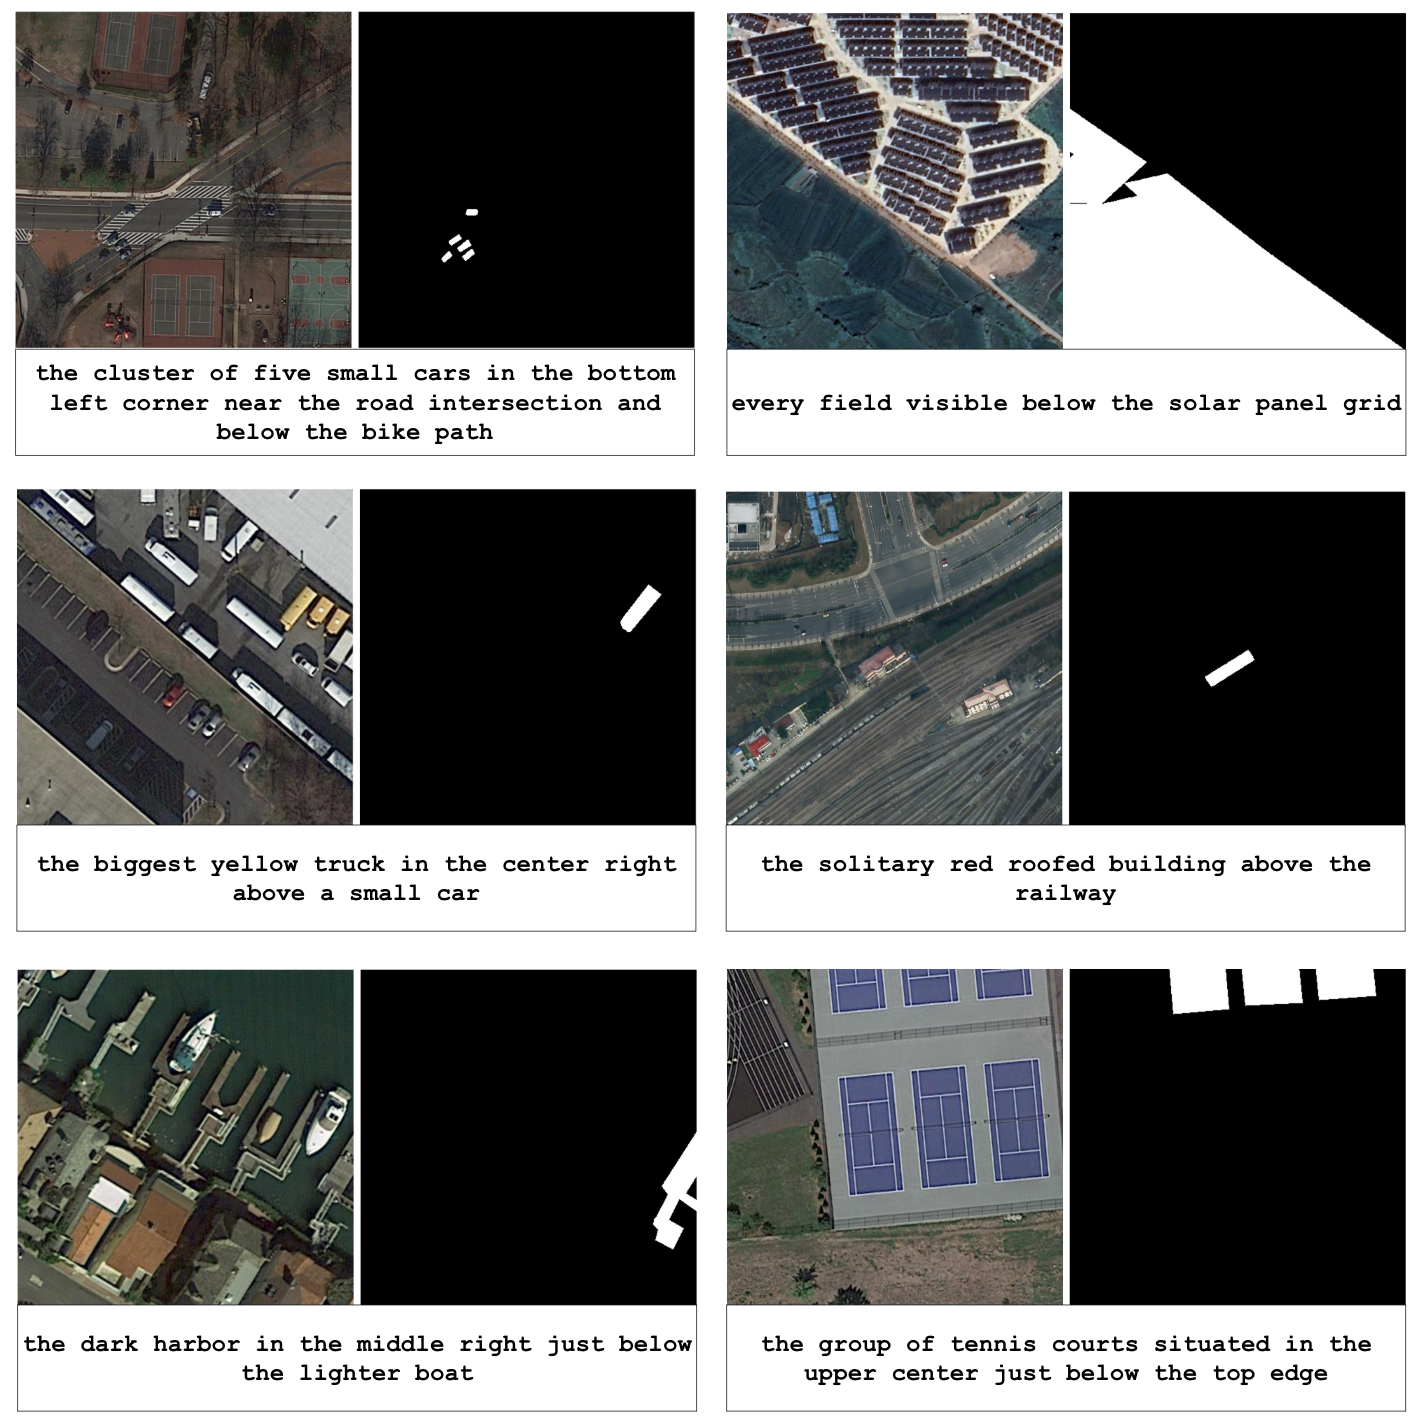
\includegraphics[width=\columnwidth]{./images/6samples.png}
\caption{Representative examples from Aerial-D dataset showing diverse referring expressions with corresponding aerial images and ground truth masks.}
\label{fig:dataset_examples}
\end{figure}

A critical component for developing effective models for RRSIS is access to high-quality datasets containing aerial photographs, precise segmentation masks, and natural referring expressions. To address this need, we introduce Aerial-D, the largest referring segmentation dataset for aerial imagery to date, comprising over 1.5 million expressions across 37,288 aerial image patches. The primary focus of Aerial-D is not only to provide exceptional training data quality but also to establish the most challenging benchmark for RRSIS to date, which will hopefully prompt research into novel RRSIS model architectures that can surpass current performance limitations.

Our key contributions include: First, we present Aerial-D, the first comprehensive large-scale aerial referring expression segmentation dataset. Second, we introduce a fully automatic dataset construction pipeline, the first of its kind to generate an entire referring segmentation dataset without manual annotation. Third, as part of this pipeline, we demonstrate how model distillation techniques using QLoRA fine-tuning can achieve substantial cost savings of thousands of dollars while approaching the performance of larger models, enabling efficient generation of the massive high-quality synthetic expressions in our dataset. Fourth, we train and evaluate a baseline model on Aerial-D and conduct cross-dataset evaluation to establish comprehensive benchmark scores for future research comparison.

